\chapter{RC Circuits} \label{chap:RC}
This project will focus on one type of circuit, RC circuits.
\\
An RC circuit is an electrical circuit consisting of resistors and capacitors. In its simplest form, it is composed of one of each. In that case a capacitor is placed in series with a resistor and a voltage input. When a voltage input is applied the capacitor charges, but if the voltage input is zero the capacitor will begin to discharge.
\\
\begin{figure}[H]
 \begin{center}
\begin{circuitikz}[american voltages]
\draw (0,0)
to[sqV, sqV=$v_{input}$] (0,2)
to (6,2)
to[short, -] (4,2)
to[C=$C$] (4,0)
to (6,0)
to (4,0)
to [resistor, R=$R$] (0,0);
\draw [>=latex', <->] (6,1.75) -- node[anchor=west] {$v_{C}(t)$} (6,0.25);
\end{circuitikz}
\end{center}
 \caption{A simple RC circuit with a voltage input, a capacitor and a resistor.}
\end{figure}
\section{Transient analysis}
\label{sec371}
To find out how the voltage of a capacitor changes over time when it is charged and discharged, a transient analysis can clarify this through mathematical operations.
\\
\\
\noindent\textbf{Discharging of a capacitor}\\
In the case of an RC circuit, KCL in section \ref{Klaws} can be rewritten as the following equation:
\begin{align}
i_{C}(t)+i_{R}(t)&=0, \nonumber \\
i_{C}(t)&= -i_{R}(t), \label{Ic-Ir}
\end{align}
where $i_C(t)$ is the current through the capacitor, and $i_R(t)$ is the current across the resistor. From \eqref{iC}, the current through the capacitor is:
\begin{align}
	i_C(t) = C\frac{dv_C(t)}{dt}.\label{iC=Cdv}
\end{align}
The equation for the current across the resistor \eqref{Ohm} can be rewritten as:
\begin{align}
	i_R(t) = \frac{v_R(t)}{R}. \label{iR=vR}
\end{align}
Inserting the definitions in \eqref{iC=Cdv} and \eqref{iR=vR} into \eqref{Ic-Ir} yields:
\begin{align*}
	C\frac{dv_C(t)}{dt} = \frac{-v_R(t)}{R}.
\end{align*}
Both sides are divided by $C$:
\begin{align}
	\frac{dv_C(t)}{dt} =-v_R(t) \frac{1}{RC}.
	\label{eq:dvC(t)}
\end{align}
From KVL, it can be derived that:
\begin{align}
	v_R(t) - v_C(t) = 0, \nonumber\\
	v_R(t) = v_C(t). \label{vR(t)}
\end{align}
Equation \eqref{vR(t)} is inserted into \eqref{eq:dvC(t)}:
\begin{align*}
	\dfrac{dv_C(t)}{dt} &= \dfrac{-1}{RC}v_C(t).
\end{align*}
The equation is now in the same form as \eqref{SDEG}, and can be solved as follows:
\begin{align}
\int \dfrac{1}{v_C(t)}dv_C(t) =& \dfrac{-1}{RC} \int dt, \nonumber \\
\ln\big(v_C(t)\big) =& \dfrac{-t}{RC} + A, \nonumber\\
v_C(t) =& e^{\frac{-t}{RC}}e^{A}.\label{V_eA}
\end{align}
Since $A$ is the constant of integration, $e^A$ is constant as well.
\\
By definition, the initial voltage of a fully charged capacitor is $v_C(0)=v_{input}$:
 \begin{align*}
	v_C(0) &= e^{\frac{0}{RC}}e^A, \\
	v_C(0) &= e^A.
 \end{align*}
Therefore $e^A = v_{input}$, and this can be inserted into \eqref{V_eA}. Furthermore $RC$ is replaced with $\tau$:
\begin{align}
\label{V_down}
\Aboxed{
 v_{discharge}(t) = v_{input}e^{\frac{-t}{\tau}}
 }
\end{align}
The function in \eqref{V_down} describes how the voltage decreases over time, when the capacitor is discharged.
\\
\\
\textbf{Charging of a capacitor}\\
In the case of an RC circuit, KVL in section \ref{Klaws} can be rewritten as the following equation:
\begin{align}
v_{input}-v_R(t)-v_C(t) =& 0, \nonumber \\
v_{input} =& v_R(t)+v_C(t), \label{V_B}
\end{align}
where $v_{input}$ is the voltage of the input source, $v_R(t)$ is the voltage across the resistor, and $v_C(t)$ is the voltage across the capacitor. 
\\
From \eqref{Ohm}, the voltage across the resistor can be expressed as $v_R(t)=i_{R}(t) R$. From \eqref{QCV} the voltage drop across the capacitor can be expressed as $v_C(t)=\dfrac{q_C (t)}{C}$. These voltage definitions are inserted into \eqref{V_B}:
\begin{align}
v_{input} =& i_{R}(t) R + \dfrac{q_C (t)}{C}. \label{Vb=IR}
\end{align}
As stated in \eqref{I=dq/dt}, current is defined as $i(t) =\dfrac{dq(t)}{dt}$, and this is inserted into \eqref{Vb=IR}:
 \begin{align*}
 	v_{input} &= \frac{dq_R(t)}{dt} R + \frac{q_C (t)}{C}.
 \end{align*}
Both sides are divided by $R$:
\begin{align}
\dfrac{v_{input}}{R} &= \dfrac{dq_R(t)}{dt} + \dfrac{1}{RC}q_C(t).\label{Vb/R} 
\end{align}
This is now a linear differential equation of the first order in the form of \eqref{FODE_form}:
\begin{align*}
\dfrac{dy}{dx}+h(x)y=g(x).
\end{align*}
This can be solved like in \cref{linethe}:
\begin{align*}
y&=e^{-H(x)}\left(\int e^{H(x)}g(x)dx+C\right).
\end{align*}
The terms in \eqref{Vb/R} represent these terms in the general solution:
\begin{align*}
y &= q_C(t),
\\
h(x) &= \dfrac{1}{RC},
\\
H(x) &= \int \dfrac{1}{RC}dt=\dfrac{t}{RC},
\\
g(x) &= \dfrac{v_{input}(t)}{R},
\\
\dfrac{dy}{dx} &= \dfrac{dq_R(t)}{dt}.
\end{align*}
Then the general solution for \eqref{Vb/R} is:
\begin{align*}
q_C(t) &= e^{\frac{-t}{RC}}\int_{0}^{t}e^{\frac{t}{RC}}\dfrac{v_{input}}{R}dt.
\end{align*}
The constant is placed outside of the integral:
\begin{align}
q_C(t) &= e^{\frac{-t}{RC}}\dfrac{v_{input}}{R}\bigg(\int_{0}^{t}e^{\frac{t}{RC}}dt+C \bigg). \label{Q_1}
\end{align}
The integral is now solved by substitution. First $u$ and $\dfrac{du}{dt}$ are defined:
\begin{align*}
u &= \dfrac{t}{RC},
\\
\dfrac{du}{dt}&=\dfrac{1}{RC},
\\
dt &=RC du.
\end{align*} 
By inserting these definitions into \eqref{Q_1}, the equation looks as follows
\begin{align*}
q_C(t) &= e^{\frac{-t}{RC}} \cdot \dfrac{v_{input}}{R}\cdot \int_{0}^{\frac{t}{RC}} R \cdot C \cdot e^u du,
\\
q_C(t) &= e^{\frac{-t}{RC}}\cdot v_{input}\cdot C\cdot \left[e^u\right]_{0}^{\frac{t}{RC}},
\\
q_C(t) &= v_{input} \cdot C\cdot e^{\frac{-t}{RC}}\cdot\left(e^{\frac{t}{RC}}-1\right),
\\
q_C(t) &= v_{input} \cdot C \cdot \left(1-e^{\frac{-t}{RC}}\right).
\end{align*} 
The voltage across a capacitor is given as $v_C(t)=\dfrac{q_C(t)}{C}$. By dividing the equation above with $C$. Furthermore $RC$ is replaced with $\tau$. The function for charging a capacitor is found:
\begin{align}
\label{V_up}
\Aboxed{
v_{charge}(t)=v_{input}\left(1-e^{\frac{-t}{\tau}}\right)
}
\end{align}
\section{RC circuit experiment} \label{c: RC_exp}
In the following section an RC circuit experiment has been conducted. A step voltage input applies current to the circuit till the capacitor is charged. The capacitor is then discharged. The voltage across the capacitor will be measured for the charge and discharge and will be compared to \eqref{V_down} and \eqref{V_up}.

\subsection{Experiment set-up}
For the experiment, an RC circuit has been constructed with the following values for the resistor, capacitor and input:
\begin{align*}
 R =& 4770\Omega, \\
 C =& 97.61nF,
 \\
 v_{input} =& 1 V.
\end{align*}
The circuit was set up as follows:
\begin{figure}[H]
	\begin{center}
\begin{circuitikz}[american voltages]
\draw
to[sqV, sqV=$1 V$] (0,2)
to[resistor, R=$4770 \Omega$] (4.5,2)

[short](3,2) to [short] (5,2)

to [short, C=$97.61 nF$] (5,0)
(0,0) to [short, -] (5,0)

(0,1) to [short, -] (0,2);
\end{circuitikz}
\end{center}
	\caption{An RC circuit with a resistor (4770$\Omega$), capacitor (97.61nF). and voltage input (1V).}
\end{figure}
\noindent
The RC circuit was constructed using the Analog Discovery 2. A representation of this can be seen in figure \ref{rc_flow}.
\begin{figure}[H]
	\center
		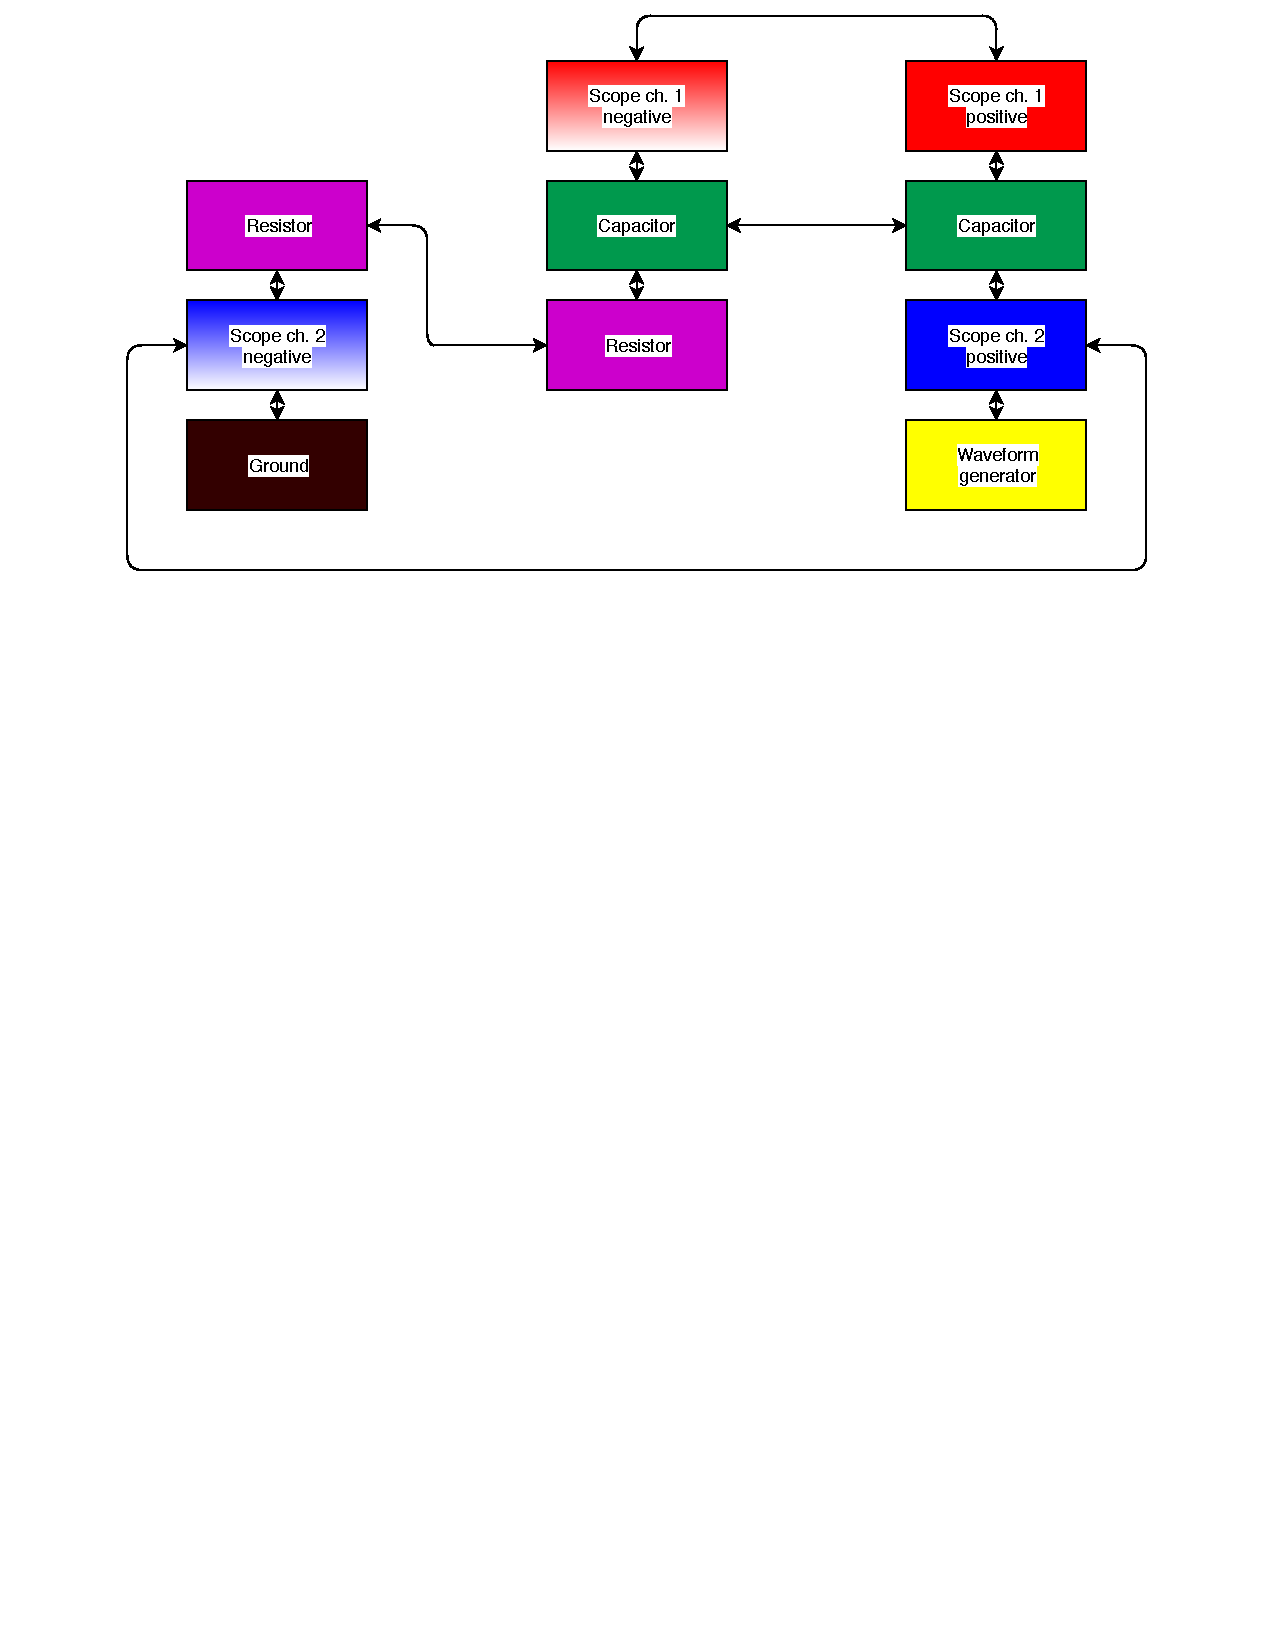
\includegraphics[clip, trim=0cm 18cm 0cm 0cm, scale=0.6]{fig/img/test_circuit_1}
	\caption{Setup of the RC circuit used in the experiment.}
	\label{rc_flow}
\end{figure}
\noindent
ANDERS FIX FIGUREN.
\\
The first step of the set-up is inserting a positive waveform generator (yellow) and a positive scope (blue) showing the waveforms. The waveform generator uses an AC step voltage. The current then passes through a resistor ($4.77 k\Omega$) and a capacitor ($97.61 nF$). Another scope is inserted to measure the charging and discharging of the capacitor. First, the current passes through a positive scope (orange), then the capacitor, and back through a negative scope (orange/white). Lastly, the current passes through a negative scope (blue/white) and into a negative waveform generator (black).
\subsection{Theoretical values}
In this experiment a step voltage input was used in which the frequency input has to be calculated. To determine this frequency one has to decide how long the capacitor should charge and discharge. To do this, a table with percentual voltage of the capacitor charges and discharges is made from \eqref{V_down} and \eqref{V_up}.
\\
After $1\tau$ the percentual voltage of the capacitor when charging can be calculated as follows:
\begin{align*}
v_{charge}(1\tau)=v_{input}\bigg(1-e^{\frac{-\tau}{\tau}}\bigg )=0.632v_{input}
\end{align*}
\\
After $1\tau$ the percentual voltage of the capacitor when discharging can be calculated as follows:
\begin{align*}
v_{discharge}(1\tau)=v_{input}e^{\frac{-\tau}{\tau}}=0.368v_{input}
\end{align*}
Below a table has been made to show how much the capacitor is charged and discharged for different $\tau$ values:
\begin{table}[H]
\center
\begin{tabular}{|l|l|l|l|l|l|l|l|}
\hline
                & $1\tau$  & $2\tau$  & $3\tau$  & $4\tau$  & $5\tau$  & $\cdots$ & $10\tau$      \\ \hline
$v_{charge}$    & $63.2\%$ & $86.5\%$ & $95.0\%$ & $98.2\%$ & $99.3\%$ & $\cdots$ & $ \sim 100\%$ \\ \hline
$v_{discharge}$ & $36.8\%$ & $13.5\%$ & $5.0\%$  & $1.8\%$  & $0.7\%$  & $\cdots$ & $\sim 0\%$    \\ \hline
\end{tabular}
\caption{The calculated percentual change in the voltage across the capacitor when it is charged and discharged at times from $1\tau$ to $10\tau$.}
\end{table}
\noindent
In this experiment firstly the capacitor charges for $10\tau$ where it is considered fully charged. The capacitor is then discharged for $10\tau$ where it is considered fully discharged. The total time the capacitor is charged and then discharged is then:
\begin{align*}
2\cdot 10\tau=2\cdot 10 \cdot RC&=2\cdot 10 \cdot 4770\Omega \cdot 97.61 nF
\\
&=9.32 ms
\end{align*} 
To get the test values compatible with the theoretical values, the frequency input has to be calculated as the hertz needed for the capacitor to charge and discharge. Therefore, the wave generator has to produce $9.32ms^{-1} = 107.3 Hz$.
\\
The data from the theoretical values and the test results can now be compared using python.
\subsection{Data comparison}
\begin{figure}[H]
\center
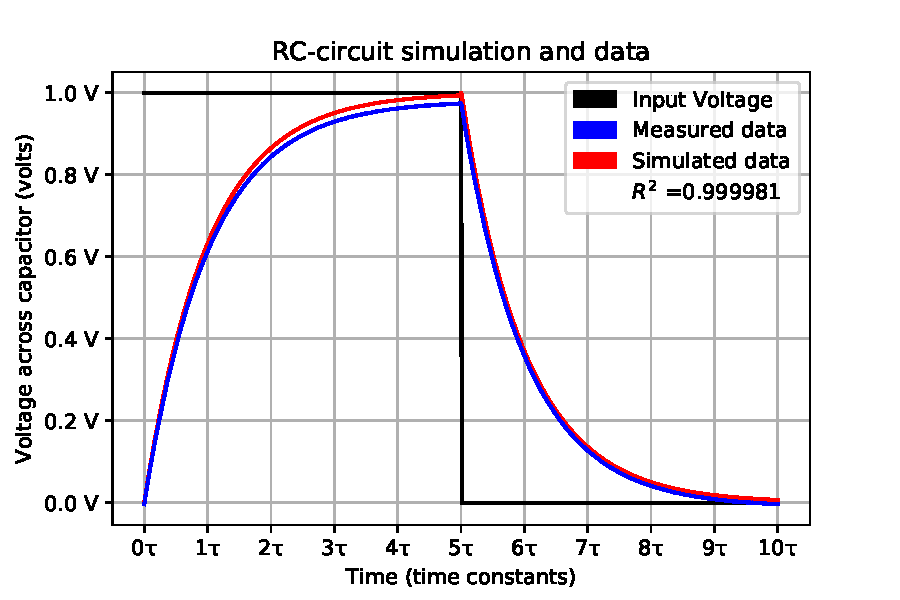
\includegraphics[scale=0.6]{fig/img/eks_1}
\caption{The measured and simulated data for the charge and discharge of a capacitor.}
\label{fig:Cap}
\end{figure}
\noindent
As shown on figure \ref{fig:Cap}, the test results are very close to the calculated theoretical values. The coefficient of determination, $R^2$, is almost equal to 1, which means that the two plots are almost identical. If the measured data was exactly the same as the simulated data, $R^2$ would be $1$. Uncertainties can be due to a few different factors. The components in the circuit might have a bit of resistance, and the capacitors integrity might not be perfect, because of usage over time, and there might be a small energy loss when running the experiment since it is not a completely isolated system. 